\Chapter{Pregunta 9}
La pregunta no. 9 tenía como propósito averiguar si los estudiantes consideraban que existe alguna relación entre la carrera de su etapa tentativa y la carrera que cursan actualmente. Por esto mismo, la pregunta era de tipo "si/no". Lo interesante se encuentra en las respuestas de aquellas personas que dijeron que sí existía una relación entre ambas carreras. \\

Debido a que las respuestas eran de tipo abierto, se analizó cada respuesta individualmente y se creó un conjunto de 5 categorías o respuestas. Dependiendo del tipo de respuesta, se colocó dentro de dicha categoría, como se muestra en el siguiente cuadro: 

\begin{center}
	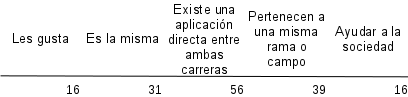
\includegraphics[scale=1]{9-cuadro1}
\end{center}

De este cuadro se nota que la mayoría de estudiantes de la muestra, que consideran que existe una relación entre carreras, proporcionan como respuesta que ambas carreras pertenecen a una misma rama o campo de aplicación o estudio, también que las carreras son la misma y además también encuentran una aplicación práctica entre ambas, siendo esta última la razón que mayor número de estudiantes tiene. \\

Con base en estos datos se procedió a analizar algunas inquietudes sobre las razones de las elecciones de carreras y las relaciones que los estudiantes encuentran. Para ello se realizaron diversas pruebas de hipótesis sobre 2 proporciones. \\

Para el primer caso, la hipótesis era que la cantidad de estudiantes de la UVG que se encuentran estudiando una carrera por que esta les gusta(P2) es mayor que la cantidad de estudiantes que ingresaron por la remuneración que les brinda la carrera (P1).\\

\begin{math}
	Ho: P_{1} - P_{2} \leq 0; 
	Ha: P_{1} - P_{2} > 0 \\
	P_{1} = \frac{89}{290}; P_{2} = \frac{16}{158} \\
	\alpha = 0.05\\
	Valor-p\leq 0.05\\
	I.C.= 0.2056 \pm 0.0709\\
\end{math}
\\
Con base en esto, se rechaza Ho; por esto mismo se concluye que el número de estudiantes que ingresaron a una carrera pensando en ser remunerados es mayor que el número de estudiantes que les gusta realmente su carrera. \\

Para el segundo caso, se deseó saber si el número de estudiantes cuya relación entre carreras es que pueden ayudar a la sociedad (P2) es mayor que la cantidad de estudiantes que ingresaron por que podían ser remunerados (P1). Este estudio es similar al anterior, ya que P2 es exactamente igual a la P2 del estudio asnterior, por lo que se concluye nuevamente que son más los estudiantes que ingresaron porque pensaban ser remunerados, que aquellos que desean ayudar a la sociedad. \\

Para el tercer caso, se deseaba conocer si la cantidad de alumnos cuya relación entre carreras era que eran la misma carrera (P2) es mayor que la cantidad de alumnos que ingresaron a una carrera por oportunidad laboral (P1). \\

\begin{math}
	Ho: P_{1} - P_{2} \leq 0; 
	Ha: P_{1} - P_{2} > 0 \\
	P_{1} = \frac{191}{290}; P_{2} = \frac{16}{158} \\
	\alpha = 0.05\\
	Valor-p\leq 0.05\\
	I.C.= 0.5574 \pm 0.072\\
\end{math}
\\
Con base en este análisis estadístico, se rechaza Ho; por esto mismo se concluye que el número de estudiantes que ingresaron a una carrera por oportunidad laboral es mayor que la cantidad de estudiantes a los que les gusta realmente su carrera. \\

Para el cuarto caso, se deseaba conocer si la cantidad de estudiantes que encuentran una aplicación en específico entre ambas carreras (P2) es mayor que la cantidad de estudiantes que les gustan los cursos específicos de su carrera (P1). \\

\begin{math}
	Ho: P_{1} - P_{2} \leq 0; 
	Ha: P_{1} - P_{2} > 0 \\
	P_{1} = \frac{184}{290}; P_{2} = \frac{56}{158} \\
	\alpha = 0.05\\
	Valor-p\leq 0.05\\
	I.C.= 0.2801 \pm 0.0929\\
\end{math}
\\
Con base en este análisis estadístico se concluye que se ha de rechazar Ho, con lo que se nota que la cantidad de estudiantes a los que les gusta los cursos específicos de su carrera es mayor que la cantidad de estudiantes que encuentran una aplicación en específico entre ambas carreras. Esto explica que no necesariamente una persona que no haya encontrado una relación entre ambas carreras no va a disfrutar la carrera en la que se encuentra, ya que si le gustan los cursos específicos de su carrera significa que al final se encuentra en un área en la que puede desenvolverse, ya que existe motivación. Además, aquellos estudiantes que sí encontraron una aplicación entre carreras podría no gustarles algunos cursos específicos. \\

Para el quinto caso, se deseaba conocer si la cantidad de estudiantes cuya relación entre ambas carreras es que les gusta realmente la carrera (P2) es mayor que la cantidad de estudiantes que ingresan a una carrera solamente por la popularidad de la misma (P1). \\

\begin{math}
	Ho: P_{1} - P_{2} \leq 0; 
	Ha: P_{1} - P_{2} > 0 \\
	P_{1} = \frac{37}{290}; P_{2} = \frac{16}{158} \\
	\alpha = 0.05\\
	Valor-p = 0.2049 > 0.05\\
	I.C.= 0.0263 \pm 0.0607\\
\end{math}
\\
Con base en este análisis, se concluye que no es posible rechazar Ho, con lo que no se cuenta con evidencia significativa para demostrar lo contrario a Ho, es decir, para demostrar que la cantidad de alumnos a los que les gusta la carrera no es mayor que la cantidad de alumnos que ingresaron por la popularidad de la carrera. Esto quiere decir que una gran parte de los estudiantes de la UVG que encuentran una relación entre carreras es más por que les gusta, en vez de dejarse llevar por la popularidad en la elección de la carrera, por ejemplo dejarse llevar porque sus amigos ingresaron a esa carrera, etc.\\

Para el sexto caso, se deseaba conocer si la cantidad de estudiantes a los que les gustaba realmente su carrera (P2) es mayor a la cantidad de estudiantes que reconocieron que sus papás les influyeron en la elección de su carrera (P1).\\
\\
\begin{math}
	Ho: P_{1} - P_{2} \leq 0; 
	Ha: P_{1} - P_{2} > 0 \\
	P_{1} = \frac{54}{290}; P_{2} = \frac{16}{158} \\
	\alpha = 0.05\\
	Valor-p = 0.009 \leq 0.05\\
	I.C.= 0.0849 \pm 0.065\\
\end{math}
\\
Con base en este análisis, se rechazó Ho, con lo que se concluye que es mayor la cantidad de estudiantes que fueron influídos por sus padres en la elección de su carrera que la cantidad de estudiantes a los que les gusta realmente su carrera. Esto puede sugerir que, de alguna forma, para aquellos estudiantes cuya relación entre carreras es que les gusta, la elección de su carrera haya sido totalmente basada en que era su sueño y que querían hacer lo que siempre habían soñado hacer y que no les importó la opinión de sus padres. Este tipo de resultado se aprecia más en estudiantes de carreras que pertenecen a facultades como Ciencias y Humanidades y Educación.


 